% \hypertarget{optical-lattice}{%
% \section{Optical lattice}\label{optical-lattice}}
% \chapter{Towards an optical lattice for quantum simulation}
% \section{Quantum $\cap$ Complexity}\label{sec:lat-introduction}
% \section{Optical lattices}\label{lat-history}
% % \subsection{Helium's promise}\label{lat-helium}
% \section{Lattice construction at ANU}\label{ssec:lat-motivation}
% \section*{Future work}\label{lat-futurework}


\chapter{Towards an optical lattice trap for helium}
    


\section{Motivation}
% keep to 1 page
	A keystone in the endeavour of physical science is the ability to foresee physical properties of substances that do not yet exist. The art and science of materials engineering dates back at least as far as early ceramic or metallurgical work. As humankind has developed more sophsticated and reliable understanding of the mechanisms underlying physical properties, so too has the design of new materials become guided more by principle and prediction than random combinatorial search. In the solid-state domain, where large numbers of constituent particles are correlated by non-negligible interactions, this project is particularly challenging because analytical models may be conceivable but analytically intractable, and the typical recourse to numerical computing is prohibited by the onerous demands on computer memory or runtime or both. Parallel to the trend of increasing precision and scale of physical models is the widening perspective of theoretical physics founded on the premise that \emph{information is physical}. Long has it been said that the workings of nature conform to mathematical language; the welcome infiltration of computer science into physical science now offers bridges from the physical to the computational. The concept of \emph{abstraction} is central in computer science and formalizes the notion of substrate-independence. This is what allows the realization of universal computing in the Von Neumann architecture, instantiated in enormous variety from the prototypical Colossus and ENIAC to the Summit supercomputer and Arduino microcontrollers. Abstracting the notion of abstraction away from computer science and into physics provides grounds for the growing field of \emph{quantum simulators}: If you care about the physics, you care about the Hamiltonian, not the objects that the summation indices refer to. The hope, then, is that one can build systems that are governed by  particular (or, perhaps, arbitrary) equations of motion such that your experimental system can generate useful data to constrain the search for new material design at a more affordable rate than conventional computing, when measured in some combination of time, energy, or some other convenient currency. One flourishing branch of this field of inquiry is the use of \emph{optical lattices} to synthesize artificial crystals, scaled up some 10,000 times and many orders of magnitude colder than conventional solids. The ultracold atoms in such systems then play the role of electrons bound in the ion lattice of solid systems. In some of these devices, the sophstication and subtlety of the experiments surpasses direct simulations of solid-state models and encroaches on the central questions about emergent complexity, fundamental particle physics and the arrow of time. For all their dizzying capabilities, optical lattices have to date relied upon only coarse measurements of momentum-space information, precluding access to detailed dynamical information such as particle currents and aspects of quasiparticle formation. Ultracold metastable helium thus offers a dramatic extension of the questions one can ask of optical lattice simulators. This chapter details the early development and ongoing efforts at the ANU \mhe group towards realizing this potential.


\begin{adjustwidth}{1.5cm}{0cm}
\begin{flushright}
\emph{``It might be noted here, for the benefit of those interested in exact solutions, \\
that there is an alternative formulation of the many-body problem:\\
How many bodies are required before we have a problem? \\
G. E. Brown points out that this can be answered by a look at history. \\
In eighteenth-century Newtonian mechanics, the three-body problem was insoluble. \\
With the birth of general relativity and quantum electrodynamics
in 1930,\\ the two- and one-body problems became insoluble. 
And within modern\\
 quantum field theory, the problem of zero bodies
(vacuum) is insoluble. \\
So, if we are out after exact solutions, no bodies at all is already too many!"}\\
 - Richard Mattuck\footnote{R. Mattuck, \emph{A Guide to Feynman Diagrams in the Many-Body Problem}, Dover Books on Physics (1992)}
\end{flushright}
\end{adjustwidth}

\section{The many-body problem}
\subsubsection*{There's always a bigger Hilbert space}

	it from bit

	The prospect of simulating one quantum system by another goes back at least as far as Feynman \cite{feynman82}, who noted in the 80s that the rapid growth of the Hilbert space with the number of objects $N$ presented a serious obstacle to computational physics. More concretely, given two quantum systems $A$ and $B$ with $d_A$ and $d_B$ degrees of freedom each, the natural way to represent the composite of the two systems is the tensor product $\mathcal{H}_C$ of their respective Hilbert spaces $\mathcal{H}_A$ and $\mathcal{H}_B$, whose basis can be written as
	\begin{equation}
		\{\ket{e_C}\} = \{\ket{e_A e_B}\} = \{\ket{a_A}\otimes\ket{e_C}\},
	\end{equation}
	where the dimension of the composite system $d_C = |\{\ket{e}\}| = d_A d_B$; a simple illustration of the resource challenge is that a system of $N$ two-level systems thus has a total dimension $2^N$. A pure state can be represented as a vector with $2^N-1$ coefficients (the asymptotically trivial reduction by 1 owing to the normalization of the wavefunction), but a general mixed state must be encoded in a density matrix while tracking $2^{2N-1}-1$  coefficients\footnote{While the density matrix has $2^N\times2^N$ entries, the normalization condition and symmetry properties reduce this slightly, but this is no general recipe for ameliorating the many-body problem.}. The Hamiltonian, if similarly stored as a full matrix, has comparable memory requirements. If the complex coefficients are to be represented by pairs of floating-point number with single precision (for 8 bytes per coefficient), the memory of a consumer-grade laptop is exhausted by the state vector of 16 two-level systems; the density matrix and hamiltoniane exceed available memory for even smaller systems. 

	Fortunately it is not always necessary to store the full state vector, density matrix, or Hamiltonian in memory. For the latter, a sparse representation suffices as most systems of interest exhibit local coupling only, and so most coupling constants are zero. However, matrix diagonalization algorithms exploit tradeoffs between memory use and compute depth, which one must confront when dealing with time-dependent problems or parametrized Hamiltonians. The memory requirements for the state vector can also be reduced for purposes of simulations by using inventive representations. A full review of numerical techniques is far beyond the scope of this thesis, but we will note that exact diagonalization \cite{zhang10} is complemented by an expanding suite of techniques including matrix product states \cite{schollwoeck11} employing the density-matrix renormalization group iterative method \cite{dechiara08}, the Multiscale entanglement renormalization ansatz \cite{}, more general tensor-network representations, quantum Monte Carlo simulations, and emerging techniques using artificial neural network representations of many-body states \cite{}. 

	Common classes of computational approach; ground-state solving (variational algorithms), time evolution, ...?
	Physical insight -> dimensionality reduction; where these not obvious, neural networks can do well...
	% -> Sometimes many-body systems are tractable because one can reduce the degrees of freedom; eg meanfield, thermodynamics in the extreme case... occasionally one is limited by insoluble equations or intractable integrals, but where exact solutions are absent sometimes asymptotically-correct approximations do OK... occasionally we are limited by ingenuity, but in general we are compression-limited in dealing with strongly-correlated systems
	% state of the art of QMC - people have done 3D bose hubbard right, and done exceptionally well. 

	Quantum-native platforms offer a route by which to circumvent some of these issues; clearly Nature has no trouble evolving the state of some $\mathcal{O}(10^23)$ spins in solid materials; if one encodes the physics of interest \emph{directly} into another quantum system, then the space (memory) requirements of simulating quantum systems is obviated. This does present another challenge, which is the means of instantiating the state and the means of implementing state evolution. Among a wide class of specialized algorithms with less obvious physical counterparts, such as prime factoring or graph partitioning, quantum simulation is within the purview of universal quantum computers. A fairly direct translation of classical techniques to digital quantum computers is \emph{Trotterization}, whereby one approximates the time evolution of the state vector
	\begin{equation}
		\ket{\psi(t)} = \hat{U}(t)\ket{\psi(0)} = \exp(-i\hat{H}t/\hbar)\ket{\psi(0)}
	\end{equation}
	by breaking the unitary evolution into iterative application of an approximate unitary operator with time step $\Delta t$ as
	\begin{equation}
		U_{k} = \exp(-i\hat{H}k\Delta t/\hbar).
	\end{equation}
	More modern and quantum-native approaches include qubitization....
	Quantum simulation basically quantum-state monte carlo for some approaches...

	As of the time of writing this dissertation, the largest digital quantum computers have around 50 qubits, and are not able to implement fault tolerant quantum computation at a physically meaningful scale. While the early results claiming a quantum advantage have made it to press, the public sphere has not been informed of any simulations of physical systems that are definitively beyond the reach of modern or near-term classical computers. Important milestones have been reached along the way in trapped ions \cite{} and superconducting cirtuits \cite{}
% various forms of isolated quantum systems... such that information doesn't leak in (unless you're building a sensor, you want your state to be independent of what's going on around it, other than your controlled inputs)
% 	Optical Nicely isolated, but (??) roadblocks?
% 		% Garanovich et al, Light propagation and localization in modulated photonic lattices and waveguides, physics reports 518, 2012
% 		% Recent xanadu paper?
% 		% Boson sampling result
% 	Trapped ion  fast and high fidelity but envt decoherence is a challenge:
% 		% Blatt et al, Quantum simulation with trapped ions, nature physics 8, 2012
% 		lanyon, universal digial sim https://science.sciencemag.org/content/334/6052/57
% 	Superconductors fast and high fidelity but envt decoherencfe is a challenge:
% 		% Houck et al, on-chip quantum simulation with superconducting circuits, nature pysics 8, 2012

	An important counterpart to universal digital quantum simulation is \emph{analogue} simulation\footnote{So called as they rely on the prinicple of controlling physical systems analogous to the systems of interest, not because of the use of analog signals as in the digital/analog dichotomy.}. The closest analogy in classical computing is the ASIC, or application-specific integrated circuit: analogue simulators are direct and dedicated simulations of a specified family of Hamiltonians for exploration of that system in particular. The prominent physical platforms for such simulation are in trapped ions \cite{}, others \cite{}, and optical lattices, which are the focus of this chapter. While schemes have been proposed for universal quantum computing with neutral atoms in optical lattices \cite{brennen99,henriet20}, this potential is still some way off \cite{markov00}. Meanwhile, analog simulation in optical lattices is flourishing. For the second time, we will note that `any attempt to produce a comprehensive review is out of date by the time it is published' and, in the below, survey some pivotal results in order to clarify the specific contributions that metastable helium atoms could make to the suite of capabilities in optical lattices.

% 	% ah yes; QMC and the sign problem...
% 	% 	that gravity paper? Sign problem is topological? But so far only a barrier to 'general' solutions?
% 	% 	\cite{ringel17} %https://advances.sciencemag.org/content/3/9/e1701758, https://advances.sciencemag.org/content/6/33/eabb8341.abstract,		https://journals.aps.org/prresearch/abstract/10.1103/PhysRevResearch.2.032060

% high energy phys models, exotic states of matter; forecast to quantum-active matter with native cellular compute... insertion of 'agents' directly into a synthetic physical envt

\subsubsection{Quantum simulation with optical lattices}

	Optical lattices found their use in cold-atom science for spectroscopic, interferometric, and atom-optical applications before they burst onto the scene as quantum simulators. However, that rich history is beyond our scope here. The first headline-grabbing experiment was the achievement of the Mott insulating state\footnote{A hallmark of the Mott insulator is the suppression of number fluctuations at each lattice site (i.e. \emph{number squeezing}), which was first observed a year prior in \cite{orzel01}. However, the later result was the first to eliminate number fluctuations in 3D - see \cite{morsch06} for discussion.} in a lattice filled with ultracold bosonic atoms \cite{greiner02}, realizing the proposition by Dieter Jaksch \emph{et al.} from three years prior \cite{jaksch98}.  The subsequent few years saw an explosion of foundational research and technical development, summarized in the reviews \cite{morsch06,bloch08}, and the following decade heralded many major advances in quantum simulation \cite{bloch12,gross17}. Theoretical foundations of the myriad models realized in lattices, and their context in a more general condensed-matter setting, are discussed in \cite{LewensteinLattices, lewenstein07}.

	The central principle of an optical lattice is the careful deployment of the optical dipole force \cite{grimm00} to `paint' a potential energy landscape with a persistent periodic structure. A stable laser is reflected back on itself, creating a standing. Atoms in this optical field thus subject to a periodic potential along the axis of propagation of the laser. For a red-detuned beam, the potential energy is minimized at the intensity maxima, providing transverse confinement as inherited by the structure of the beam. If the lasers are in the TEM(0,0) mode, the Gaussian profile provides an approximately harmonic confinement when the kinetic temperature is small. At ultralow temperatures, the site-to-site variation of the potential energy is nearly constant. Additional laser beams can break the axial symmetry and induce two- or three-dimensional periodic structures. The simplest of these is a square lattice, but more complicated geometries can be realized by different optical arrangements. Hexagonal honeycomb \cite{jotzu14} and triangular geometries complete the simple tiling structures in 2D, which is extended by the Kagome lattice and the recently-emerging quasicrystal lattices. Disorder can be introduced to intentionally break translational symmetry by superposing the speckle pattern of another laser or by collinear propagation of another laser whose wavelength is close to an irrational multiple of the main lattice. 

	An ever-expanding suite of additional allow the experimentalist to furnish their lattices with sophisticated control over the dynamics. For example, by synthesizing complex coefficients in the coupling constants between neighbouring sites, neutral atoms can be made to mimic the motion of charged particles in electromagnetic fields. Such synthetic fields underpin the realization of numerous paradigmatic consended-matter models \cite{aidelsburger13,tai17,endres11,rispoli19,jo09,simon11,miyake13,folling07,jotzu14}. Efforts are ongoing to extend the reach of the cold-atom lab to simulations of high-energy phenomena like matter coupled to non-abelian gauge fields \cite{zohar16,schweizer19,tagliacozzo13} and the Schwinger effect of particle-antiparticle pair production. Through varying parameters such as the ratio of the tunnelling and interaction energies (the latter often achieved via Feshbach resonances), optical lattices permit direct realization of quantum phase transitions \cite{greiner01,eckardt05,jordens08,jo09,haller10,simon11,baumann10,leonard17,landig16,sachdevQPT,endres12,anquez16,clark16} and topological phase transitions \cite{goldman16,nakagawa14}. The former occurs when the ground state of a Hamiltonian of the form $H = H_0 + g H_1$ assumes a different character on either side of some critical value $g_c$. The latter is concerned emergence of a nonlocal order parameter capturing the long-range entanglement structure inherent in different topological phases.

	Modern work in lattices also permits direct inquiry into the role of entanglement in many-body systems out of equilibrium \cite{amico08,eisert15}. Direct observations of the growth and propagation of entanglement coincident with the onset of thermalization \cite{clos16,kaufman16} from an initially pure state cement principles of quantum information into the foundations of thermodynamics \cite{osborne02,osterloh02,isakov11,jiang12,dalessio16,goold16,srednicki94}. Further outlining this connection is the utility of so-called `algorithmic cooling' whereby high-entropy portions of the many-body quantum state are explicitly identified and removed \cite{bakr11,rodriguez-briones17,boyin02}. The application of disordered and quasirandom lattices has permitted direct inquiry into wavefunction localization \cite{anderson58,dalessio16,goold16,srednicki94,clos16,kaufman16}, wherein the presence of disorder prevents the system from thermalizing and instead retains local information about its initial state over long timescales.

\subsubsection{Quantum state microscopy}

	A key enabler of the myriad studies described above are the techniques of quantum gas microscopy \cite{bakr09,cheuk15,endres11,haller15,miranda15,parsons15,rispoli19,sherson10,miranda17,preiss15a} including single-site measurements of spin and particle parity (and recently even population up to $N=4$ \cite{preiss15a}). These techniques also permit site-resolved state preparation. Direct access to microscopic information renders density correlations readily measurable \cite{endres11,rispoli19}, and sophisticated interferometric techniques even resolve the degree of entanglement (via the R\`{e}yni entropy) between sites \cite{brydges19,daley12,mouraalves04,palmer05}. One aspect which has otherwise been absent from the cold atom toolbox is \emph{momentum microscopy}, as afforded by metastable helium. During the course of my PhD, a helium lattice was constructed, and achieved the Mott insulating state, at the Institut d'Optique in Palaiseau \cite{ClementLattice}. As shown by the abundance of research based on site-resolved microscopy, as described above, there is a wealth of study that could be done with access to microscopic momentum information; more than one machine will surely not be enough to cover all the interesting ground. Moreover, the existence of independent apparatus will permit independent replication of experiments that might yield highly surprising results. The remainder of this chapter deals with the particular prospects, and progress towards, an optical lattice for ultracold metastable helium at the ANU.


		Correlation functions factorize in simple cases; Bethe ansatz when things reduce to 2 body??
		Experiment exploit corrfuns 
			\cite{schweigler17}
			\cite{hodgman17}

			Single atom detection
	\cite{ott16} review - entirely position-space?


\section{Realizing the Bose-Hubbard model}
	\cite{grimm00}% optical dipole traps 
	\cite{miller93}% Far-off-resonance optical trap- ping of atoms,” Phys. Rev. A 47, R4567–R4570 (1993).
	\cite{barrett01}% “All-Optical Formation of an Atomic Bose-Einstein Condensate,” Phys. Rev. Lett. 87, 010 404 (2001).
	\cite{cabrera}%-gutierrez18 calibration by sudden phase shift of trapping beam; similar in spirit to trap freq measurements in earlier chap
	\cite{celi14}% proposes use of quantized internal states as an additional lattice dimension, but we would prefer to opt for spatial dimensions here
	\cite{gadway18}% momentum spae lattice even proposed
	\cite{ghose03}% magneto-optical lattice for studies of quantum chaos
	floquet prob worth mentioning?
		perhaps move these alt models up with discussions of various geometries 
	\cite{hooley04}
		difference in density of states due to presece of harmonic potential, even in the strength->0 limit
	\cite{kastberg95}
		lattices briefly held the record for the lowest kinetic temperature record; early (temporary) confinement?
		lattice potentials were actually used a fair bit (eg depletion paper) well before Mott insulator transition realized, which catapulted them into the forefront of the physics community
	\cite{machholm03}
		band structure and excitations of BEC in optical lattice (early work; what did this do first??);
		bloch solns (as in machholm03) are unstable and give way to soliton trains machholm04
	ditto, two level atom in periodic optical potential
		\cite{wilkens91}
	introduction to maximally localized wannier fns
		\cite{marzari00}
	\cite{pavarini11}
		wannier fns tutorial
	original wannier paper
		\cite{wannier37}
	\cite{peik97}
		Early use of lattice for kapitza-dirac scattering?? bloch oscillations of atoms in optical potentials



	\begin{figure}[h]
	\centering
	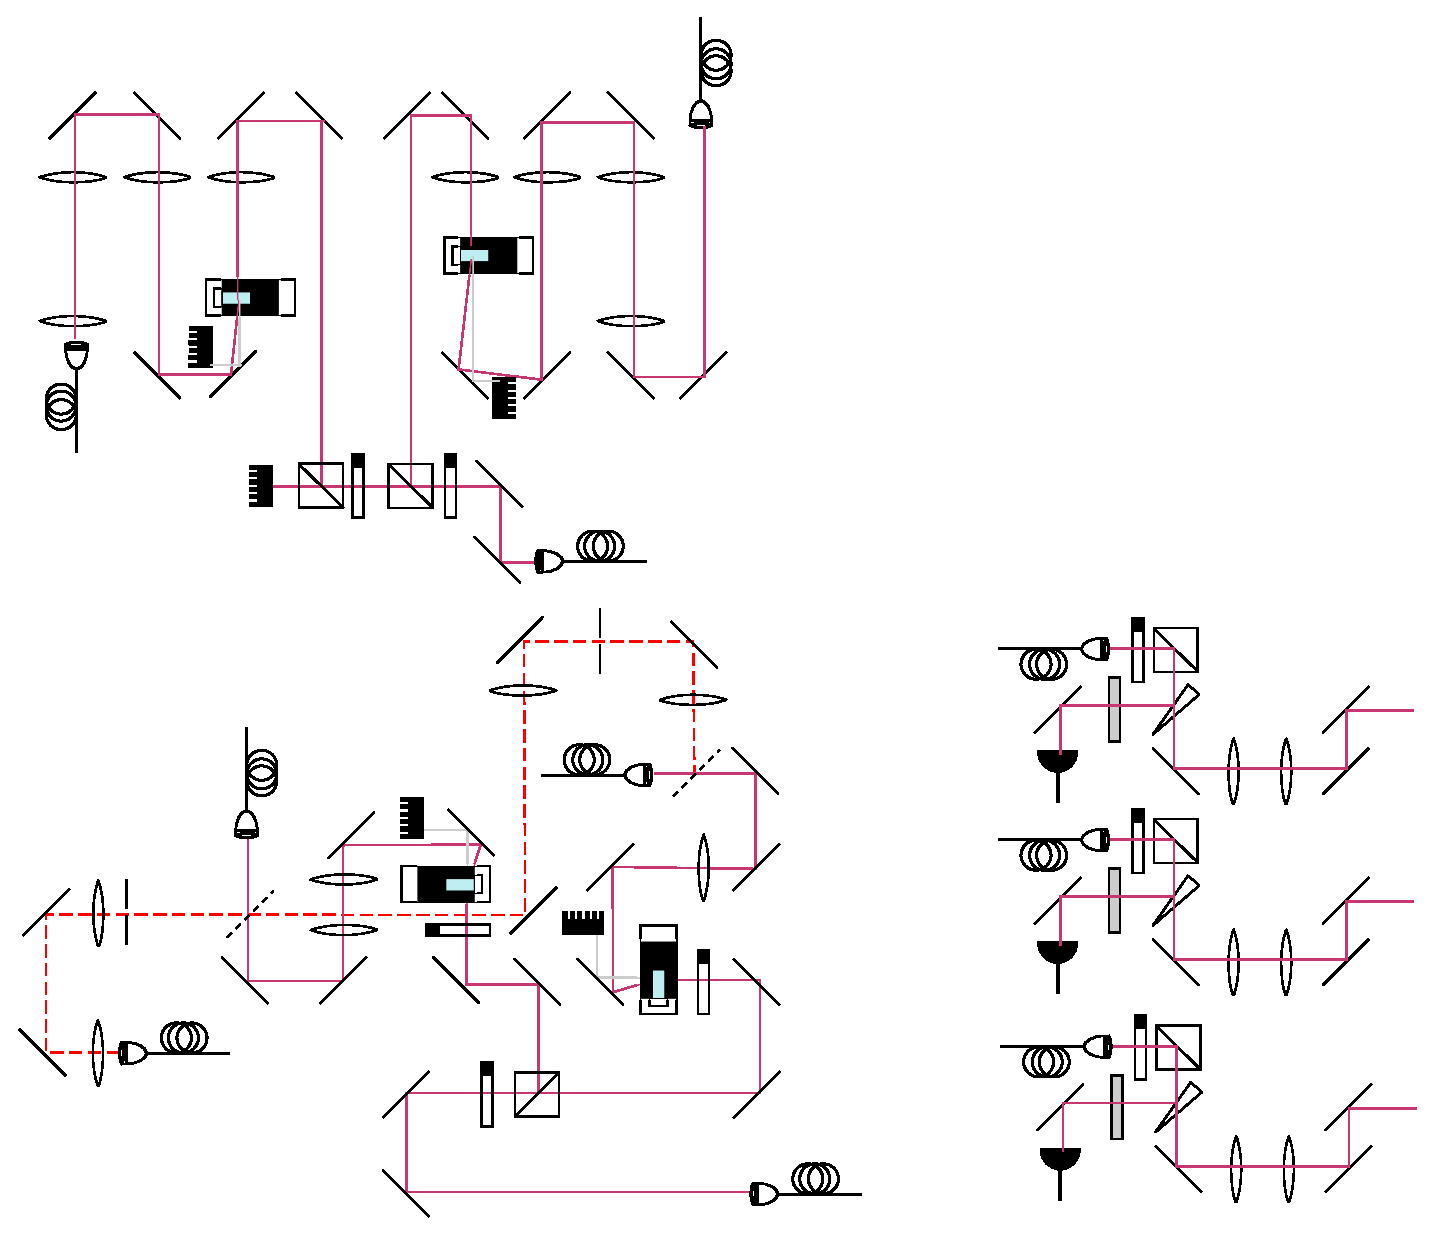
\includegraphics[width=\textwidth]{fig/apparatus/dipole_optics}
	\caption{Schematic 1550nm optics used in the upstairs experiment.}
	\label{fig:dipole_optics}
	\end{figure}

\subsection{Wannier functions}


\section{Construction of experimental apparatus}

\begin{adjustwidth}{1cm}{0cm}
\begin{flushright}
\emph{``It is not necessary to succeed in order to persevere. As long as there is a margin of hope, however narrow, we have no choice but to base all our actions on that margin"}\\
- Leo Szilard\footnote{\emph{LIFE magazine} volume 51, issue 9, 1961 }\\
\end{flushright}
\end{adjustwidth}

This experiment did not start from scratch: An existing helium beamline and MOT chamber formed the foundation for the rest of the construction. After some years of disuse, the optics were dirty and certainly required realignment or replacement. The optical distribution hardware was present but not functional. This section documents the extensions I built towards the goal of reaching BEC in this machine

\subsection*{Infrastructure upgrade}

\subsubsection{First MOT}
\subsubsection{Vacuum system renovation}
% wiki/December_2018_Bake
% wiki/Mid-December_2018_Bake
\subsubsection*{Absorption imaging}

While the greatest comparative advantage of helium, with respect to other atomic species, is the far-field detectability via the MCP-DLD, the more conventional technique of absorption imaging is of great utility for diagnostics. Principally, direct imaging of atoms in traps is possible, and the possibly large field of view means rather hihg-temperature clouds can be detected. In our apparatus, the absorption imaging setup was particularly advantageous because we were unable to install the MCP-DLD for some time as we were waiting for parts to be machined. Meanwhile, absorption imaging proved to be instrumental.

A simple characterization of absorption imaging is that one `takes a photo of the shadow of the atoms' by illuminating the sample with a collimated laser beam, and then projecting the beam onto an appropriate sensor. In our apparatus we used a Bobcat model camera manufactured by Xenics. The photosites are InGaAs substrate with a 20 $\mu$m pixel pitch, and a 320x256 pixel sensor array. The camera received light from the absorption imaging setup depicted in Fig. \ref{fig:abs_img}. Detailed discussions of the physical principles of this technique are presented in \cite{MakingProbingUnderstanding,TychkovThesis}. Here we present a simple picture.

A laser tuned close to resonance with the atomic sample is coupled via optic fibre to the absorption imaging setup. The light passes through a polarizing beam splitter and then a half-wave plate to set the polarization, which is useful when imaging in the presence of a bias field. The beam is then magnified by a 4:1 telescope to a $\approx1$ cm waist and directed at the atomic sample through the vacuum windows. Light on the exit side of the cloud will have been attenuated by a factor $e^{i\phi}A$.  The attenuation factor $A=\exp(-\frac{\tilde{n}\sigma_0}{2}\frac{1}{1+\delta^2})$ depends on the column density integrated along the beam axis $\tilde{n} = \int n(x) dx$, the detuning $\delta=2(\omega-\omega_0)/\Gamma$ of the laser from resonane as measured in half-linewidths, and the absorption cross-section which is $3\lambda^2/2\pi$ in the two-level approximation. The phase $\phi$ also depends on the atomic density and detuning from resonance, and is in principle useful for techniques like phase contrast imaging, but is not presently used in our experiment. The light intensity is recorded by the camera in an exposure time of XXXms in our system. The resulting `shadow' image is then followed, within a few milliseconds, with a second laser pulse. By this point the atoms have scattered many photons and left the laser path. The second image is used as a reference to compute the absorption along each column delineated by the edges of the pixels. A light-free image can be used as a `darkfield' to reduce the camera's inherent noise profile. The pixel-wise absorption is then found by
\begin{equation}
	\frac{I_\textrm{abs}-I_\textrm{dark}}{I_\textrm{ref}-I_\textrm{dark}}:=t^2(x,y),
\end{equation}
which can be processed by appropriate filtering or smoothing to remove image artefacts. The 2D absorption profile can be fitted for further quantitative analysis for purposes of thermometry or determining the atomic population.
% http://www.heliumbec.com/wiki/2017/05/09 - first image?
% wiki/2017/05/31  alignment using vertical BOBCAT creating the 'helium comet'

\subsubsection{Second MOT \& Magnetic trap}
% http://www.heliumbec.com/wiki/2017/02/10
% http://www.heliumbec.com/wiki/2017/04/04
% http://www.heliumbec.com/wiki/2017/06/22
% wiki 2017/06/05 some OK image of magnetic trap; may do better
% wiki/Magnetic_trap no imgs but an old lifetime measurement; looks bad, must have had high pressure
\subsubsection{Dipole trap}
% more detail about these. Some examples of absorption imaging results.
% http://www.heliumbec.com/wiki/2017/05/19
	% The saturation intensity of the transition is 0.16 mW/cm$^2$. Our imaging power is well below this.
% We observe a weird problem that when the RF evaporator is set to the initial 500ms of 34MHz constant radiation, the frequency to the vertical dipole AOM shifts, causing the beam to move far enough that it no longer hits the fibre. Further investigation show that this effect is present between 34-38MHz, but seems to disappear for 33MHz and below as well as 40MHz. Oddly though, for the higher initial frequencies when the ramp is swept through the trouble region we see no deviation (although it might be too quick to observe). Anyway, for now we just set the initial frequency at 33MHz and move on, and will investigate further some other day.
% LOL
% http://www.heliumbec.com/wiki/2017/07/03 first crack sighting

% http://www.heliumbec.com/wiki/2017/07/04 beam profiling
% http://www.heliumbec.com/wiki/2017/08/14 pesky ion signals..
% http://www.heliumbec.com/wiki/2017/08/16 better traces
% evidence against dipole nature; various 'maxima', short steps led to large variation, diminishing peak shape over consecutive runs despite stable alignment and power etc - eventually found unexpectedly high N2 and CO2, perhaps some organic compound 'ablating' from the laser heat http://www.heliumbec.com/wiki/2017/10/20
% http://www.heliumbec.com/wiki/2017/10/26 first sighting of dipole - abandoned idea of optimizing on ion signal and just took a ton of images while stepping through focus lens posn
% http://www.heliumbec.com/wiki/2017/10/27 img simultaneous with resonant exposure, nice narrow beam, shows diff posn to dipole -> diff refractive index
% http://www.heliumbec.com/wiki/2017/11/20 vert alignment?
% http://www.heliumbec.com/wiki/2017/11/28 vert resonance
% http://www.heliumbec.com/wiki/2017/11/22 horz resonant beam with properly alignd img beam (straight channel)
% http://www.heliumbec.com/wiki/2017/11/24 img of double dipole
% http://www.heliumbec.com/wiki/2017/12/01 nice single dipole? pics
\subsection{Subsequent progress}
\section{Future work}
\subsection*{Construction}

Well, dipole, maybe better automation, certainly better envt controls... 
\subsection*{Scientific aims}

\section*{Workspace}


		
	Often used in conjunction with eg. feshbach resonance 
	have their own noise sources
		\cite{pichler10}% nonequlibrium dynamcics of bosonic atoms in optical lattices: Decoherence of many-body states dues to spontaneous emissions
	Complex potentials with additional optical fields, creating synthetic gauge fields
		\cite{aidelsburger11,aidelsburger13,miyake13}


* Cut my teeth on AO alignment and eventually building
a MOT with an old-school security camera * Assembling new vacuum system
Construction Bakeouts - logs? Ti Sub and NEG improvements * LVIS * MOT 2
* Absorption Imaging * Dipole alignment * Misadventures and eventual
fluke - thanks to Patrick
Vacuum chamber

Optics build inc dipole So when I started, we actually didn't have a
working MOT. THere were the optis but they were dirty and eyah. So they
didn't have light either. Had to build a few AO arms - everything except
the collimator and zeeman slower I think, and the ZS was set up
according to the old paper about that lab, right? THe `optimized' one.
Altough one could certainly design a chirped system to increase yield,
but then I wonder what the density/number limits for a MOT are. How much
could we actually obtain, given that we then have to push through the
feed hold into another chamber? SO yeah. Two MOTs. Anythign exciting to
write about? Maybe not - just ballpark the capture velocities maybe. The
dipole diagram and control woudl be worth describing. The theory of
dipole trapping would belong here as it's not really relevant? Oh, no,
I'll have to put it in the alignment chapter - well it realyl sits in
the polz part of the tuneout chapter. So that'll cover that I guess.
Look over the simulations of the dipole potential. Maybe some
simulations of evaporative cooling in the dipole. Open source 'em of
course. Would be a fun way to try some auto-optimization algorithms for
path optimization. Another way to burn some time, I guess, there are a
lot of things in here that are becoming big to-do items! Bu Sequence up
to evap \& dipole Imaging system Diagram, some example images and
calculation of number Small simulations \#\# Progress meanwhile\\
New coils, solder catastrophe, new plates \#\# Issues/What next
Stability: Vibration, temp, vacuum Optics: Power, profile Automatic
optimization Broad goals Fermions Quasirandom lattices Are these
actually resources or what? Next generation laser tech?

Condensed matter models/phenomena; 
	\cite{aidelsburger13}% Realization of the hofstatder hamiltonian with ultracold atoms in optical lattices, phys rev lett 111, 2013
	\cite{tai17}% microscopy of the harper-hofstadter model
	\cite{endres11}% Endres et al, observation of correlated particle-hole pairs and string order in low-dimensional Mott insulatros, science 334, 2011
	\cite{rispoli19}% quantum critical behaviour at the MBL transition
	\cite{jo09}%, itinerant ferromagnetism in a fermi gas of ultracold atoms
	\cite{simon11}%, quantum simulation of antiferromagnetic spin chains in an optical lattice
	\cite{miyake13}% - Hofstader-Harper hamiltonian, realizes a topological insulator that breaks time reversal symmetry, ie a quantum hall insulator -> spintronics
	\cite{folling07}% evidence of microscopic effects 2nd order tunnelling
Bose-Hubbard model
	\cite{ramakumar07}%		numerical study of thermodynamics; exactly diagonalized up to 3D (!) up to 1000 atoms in 1000 sites (!!!) in 1D, 540 sites and 3840 bosons in 2D, and 2500 bosons in 50^3 3D lattice.		how??? supercomputer or smart numerics?
	\cite{freericks94}% phase diagram 
	\cite{hopjan20}% MBL in 1D		numerical paper
	\cite{jaksch05}% 'cold atom hubbard toolbox'		predates gauge field, gas microscopes, dipoles...
	\cite{larcher11}% momentum-space localization in incommensurate lattices (aubry-andre model)
	\cite{rispoli19}% disordered BHM
Phase transitions; classical, quantum, topological, dynamical
		\cite{greiner01}% uantum phase transition from a superfluid to a mott insulator in a gas of ultracold atoms, nature 415
		\cite{eckardt05} transition can also be induced by periodic driving
		\cite{jordens08}% a Mott insulator of fermionic atoms in an optical lattice
		\cite{jo09}%, itinerant ferromagnetims in a fermi gas of ultracold atoms;	emergence of ferromagnetic scale in a gas, not a lattice, with repulsive interactions
		\cite{haller10}% pinning quantum phase transition for a Luttinger liquid of strongly interacting bosons
		\cite{simon11}% quantum simulation of antiferromagnetic spin chains in an optical lattice
		\cite{baumann10}%  Dicke quantum phase transition with a superfluid gas in an optical cavity;Open system, light-matter interactions
		\cite{leonard17}% supersolid formation in a quantu mgas breaking a continuous translational symmetry, nature 543
		\cite{landig16}% quantum phases from competing short- and long-rante interactions in an optical lattice, nature 532
		\cite{sachdevQPT}%, Quantum phase transitions, cambridge univ press
		\cite{endres12}% Higgs mode in SF/MI transition
		\cite{anquez16}% quantum kibble-zurek mechanism in a spin-1 bose-einstein condensate
		\cite{clark16}%, universal space-time scaling symmetry in the dynamics of bosons across a quantum phase transition
		\cite{goldman16}% review of topologial matter in optical lattices
		\cite{nakagawa14}% - non-equilibrium, topological phase transition... 
		% L D Landau 1937, on the theory of phase transitions, Zh Eskp Teor Fiz 7
Out-of-equilibrium physics
		\cite{eisert15}% review quantum many-body systems out of equilibrium, nature physics 11, 2015
	HEP/particle/novel physical synthesis
		\cite{keilmann11}% proposal for creation of anyons in 1D?
		lattice gauge theories
			proposal
				\cite{zohar16}%
			experiments
				\cite{schweizer19}%, gorg19
		in the pursuit of non-abeliean gauge theories to study quark confinement etc
			\cite{tagliacozzo13}% - optical lattice of rydberg atoms
molecules in lattices
		\cite{yan13} dipolar spin-exchange in lattice confined polar molecules
		\cite{yang19} molecular feshbach resonances
		\cite{yan20} ultracold dipolar molecules with microwave-dressed resonant interaction; enhances interaction above s-wave scattering limit for controlled interactions and immediately applicable in lattices
		\cite{balakrishnan16} review of cold chemistry 
		\cite{yelin06, micheli06} %proposals for QC in dipolar molecules in lattices
foundations
	Thermalization/emergence of thermodynamics
		\cite{anderson58}% anderson localization in random lattices 
		\cite{dalessio16}%, from quantum chaos and eigenstate thermalization to statistical mechancis and thermodynamics, advances in physics 65, 2016
		\cite{goold16}% role of quantum information in thermodynamics
		\cite{srednicki94}% chaos and quantum thermalization, phys rev E 50, 1994
		\cite{clos16}% time-resolved observation of thermalization in an isolatd quantum system, - uses trapped ions
		\cite{kaufman16}%, quantum thermalization through entanglement in isolated many-body systems, science 353, 2016
		Coerent superposition and statistical distributions RSP
			Differentiate between them by the presence of off-diagonal terms in the density matrix - accessible by interferometry (put things in superposition) or changes of basis, right? and captured formally by purity, related to VNE 
	Role of entanglement in the emergence of entropy; many-body information (VNE); ETH/MBL
		\cite{kaufman16}%, quantum thermalization through entanglement in isolated many-body systems, science 353, 2016
		\cite{nandkishore15}% review: many-body localization and thermalization in quantum statistical mechanics, annaual review of condensed matter physics 6
			VNE and the quantum breaking of additive entropy
		\cite{chiu18}%	'direct' measurements of entropy
Jaynes; how much info in a quantum state? landauer; that thesis; 
Entanglement in many-body structure
	\cite{amico08} review 
	Entanglement is a thing!%,	Aspect et al 1982 experimental test of bell's inequalities using time-varying analysers,	Aspect et al 1981 experimental tests of realistic local theories via bell's theorem,	Giustina et al, 2015 significant loophole-free test of bell's theorem with entangled photons,	Hensen et al 2015, loophole-free bell inequailty violation using electron spins separated by 1.3km, nature 562,	Shalm et al, 2015 strong loophole-free test of local realism, phys rev lett 115
	Realism vs locality in many-body systems?
		\cite{osborne02}% entanglement in a simple quantum phase transition, phys rev A 66, 2002
		\cite{osterloh02}%  scaling of entangement cose to a quantum phase transition ??
			shows scaling behaviour in analog to correlation functions at classical phase transitions
		\cite{amico08} entanglement in many-body systems, rev mod phys 80, 2008
	local order parameters not obviously applicable to (eg) quantum hall states RSP 
		\cite{jiang12}%, identifiying topological order by entanglement entropy, nature physics 8
	or spin liquids , but non-local entanglement works. 
		\cite{isakov11}% topological entanglement entropu of a bose-hubbard spin liquid
			numerical paper on kagome lattice
		\cite{jiang12}%
			numerical study on kagome lattice
	While repeatability of ions and qubits means one can exhaustively computer the density matrix , 
		\cite{neill16}% ergodic dynamics and thermalization in an isolated quantum system
		% Haffner et al, scalable multiparticle entanglement of trapped ions, nature 438
	no known state tomography for lattices of itinerant particles, 
	and instead interferometry techniques are employted, usually by realizing identical copies in parallel
		\cite{brydges19}%  probing reyni entanglement entropy via randomized measurements, science 364
		\cite{daley12}% theoretical proposal: measuring entanglement growth in quench dynamics of bosons in an optical lattice
			using parallel copies and like-site parity measurements to determine reyni entropy
		\cite{mouraalves04}% multipartite entanglement detection in bosons, phys rev lett 93
		\cite{palmer05}% detection and characterization of multipartite entanglement in optical lattices
	Collision of quantum information and condensed matter and computing...
		\cite{bakr11}%	Realization of algorithmic cooling in lattices 
		\cite{rodriguez-briones17}% and exploting interactions for deeper cooling
		\cite{boyin02}% first implementation using NMR spins


gas microscopes; 
	\cite{bakr09}  quantum gas microscope for detecing single atoms in a hubbard-regime optical lattice
	\cite{cheuk15}  quantum-gas microscope for fermionic atoms
	\cite{endres11} observation of correlated particle-hole pairs and string order in low-dimensional Mott insulatros, science 334, 2011
	\cite{haller15}  single atom imaging of fermions in a quantum gas microscope, nature physics 11
	\cite{miranda15} site resolved imaging of ytterbium atoms in a two-dimensional optical lattice phys rev A
	\cite{parsons15} site-resolved imaging of fermionic 6Li in an optical lattice phys rev lett 114
	\cite{rispoli19} quantum critical behaviour at the MBL transition
	\cite{sherson10} single-atom resolved fluorescence imaging of an atomic Mott insulator
	\cite{miranda17} achieve imaging without the laser-cooling required to keep atoms pinned during fluorescence; extends possibility to other species
	\cite{preiss15a} - QGM of bosonic 87Rb, but with two planes resolvable, enabling number measurements beyond parity -> greater dyn range in density correlations
facilitating quantum-state engineering
	\cite{chiu18}%
	\cite{kozlowski17}% proposal for unconventional state engineering via weak measurements
	\cite{preiss15a}% - actually a quantum walk demonstration; somewhere there's a paper showing you can do UQC with walks on strange graphs...
correlation funs
	\cite{endres11}%, observation of correlated particle-hole pairs and string order in low-dimensional Mott insulatros, science 334, 2011
	\cite{rispoli19}% quantum critical behaviour at the MBL transition